\documentclass[a4paper, 12pt, fleqn]{article}
\usepackage[utf8]{inputenc}
\usepackage{graphicx}
\usepackage[T1]{fontenc}
\usepackage{amssymb}
\graphicspath{ {images/} }
\usepackage[a4paper,left=.8in,right=.8in,top=1in,bottom=1in]{geometry}
\setlength\oddsidemargin{\dimexpr(\paperwidth-\textwidth)/2 - 1in\relax}
\setlength\evensidemargin{\oddsidemargin}
%\setlength\oddsidemargin{-.875in}
%\setlength\evensidemargin{-.875in}
\usepackage{tikz}
\usetikzlibrary{positioning,shapes,fit,arrows}
\definecolor{myblue}{RGB}{56,94,141}
\usepackage{fancyhdr}
\usepackage{booktabs}
\usepackage{mathtools}
\usepackage{amsmath}
\usepackage{etoolbox}
\usepackage[hidelinks]{hyperref}
%\apptocmd{\thebibliography}{\csname phantomsection \endcsname \addtocontentsline{toc}{chapter}{\bibname}}{}{}
\usepackage{caption}
\usepackage{float}
\floatstyle{boxed} 
\restylefloat{figure}
\pagestyle{fancy}
\fancyhf{}
\fancyhead[LE,RO]{}
\fancyfoot[CE,CO]{}
\fancyfoot[LE,RO]{\thepage}

\begin{document}
 
\begin{titlepage}
    \begin{center}
        \vspace*{1cm}
        \par
        \large
                \textbf{Pune Institute of Computer Technology}	
                \linebreak
		\textbf{Dhankawadi, Pune}
        \vspace{0.5cm}
        \linebreak
        \vspace{0.5cm}
        \large
        \\Breast Cancer Classification
        Using Support Vector
        Machine 
        \linebreak
        \linebreak
		
		%\vspace{0.2cm}
		\textbf{SUBMITTED BY}
		\vspace{1cm}
		
         Rajwinder Singh (41152) \\
         Sahil Singh (41155) \\
         Sanchit Raina (41157)
        \linebreak
        \linebreak
		        
        \textbf{\large{Under the guidance of}}
		\linebreak
	    Prof. Rutuja A. Kulkarni
		\linebreak
      %  \vfill
        
        
        
        \vspace{0.8cm}
        

        
\includegraphics[scale=0.6]{pict}   
        
        \Large
        DEPARTMENT OF COMPUTER ENGINEERING\\
		\textbf{Academic Year 2021-22}
        
    \end{center}
\end{titlepage}
\pagebreak

\newpage

\section*{}
\textbf{Title:} SQL Injection attacks and Cross-Site Scripting attacks \\

\noindent
\textbf{Problem Statement:} \\
SQL Injection and Cross-Site Scripting attacks 
SQL Injection attacks and Cross -Site Scripting attacks
are the two most common attacks on web application. Develop a new policy
based Proxy Agent, which classifies the request as a scripted request or query
based request, and then, detects the respective type of attack, if any in the
request. It should detect both SQL injection attack as well as the Cross-Site
Scripting attacks. \\

\noindent
\textbf{Objectives:}
\begin{itemize}
	\item Learning and demonstrating about SQL injection attack.
	\item Learning and demonstrating XSS attacks. \\
\end{itemize}

\noindent
\textbf{Outcomes:} \\
We were able to:
\begin{itemize}
	\item design a website where SQL Injection works.
	\item design a website where XSS attack is possible.
	\item design a website that detects XSS attacks and prevent it as well. \\
\end{itemize}

\noindent
\textbf{Software and Hardware Packages:}
\begin{itemize}
	\item Django 4.0.2 
	\item SQLite Database
	\item Python 3.8
	\item Pycharm IDE
	\item OS: Ubuntu 20.04 (64 bits) \\
\end{itemize}

\newpage
\section*{}

\textbf{Theory concept with algorithm:} \\

\noindent
\textbf{SQL Injection:} \\
SQL injection is a technique used to exploit user data through web page
inputs by injecting SQL commands as statements. Basically, thesestatements can be used to manipulate the application’s web server by
malicious users. \\

\noindent
SQL injection is a code injection technique that might destroy yourdatabase.
SQL injection is one of the most common web hacking techniques.
SQL injection is the placement of malicious code in SQL statements, via web page input. \\

\noindent
Exploitation of SQL Injection in Web Applications: \\
Web servers communicate with database servers anytime they need to
retrieve or store user data. SQL statements by the attacker are designed
so that they can be executed while the web-server is fetching content from
the application server. It compromises the security of a web application. \\

\noindent
Example of SQL Injection \\
Suppose we have an application based on student records. Any student
can view only his or her own records by entering a unique and private
student ID. \\
Suppose we have a field like below: \\
student\_id: \\
And the student enters the following in the input field: \\
12222345 or 1=1. \\

\noindent
So this basically translates to: \\
SELECT * FROM students WHERE \\
student\_id = 12222345 or 1 = 1 \\
Now this 1=1 will return all records for which this holds true. So basically,
all the student data is compromised. Now the malicious user can also
delete the student records in a similar fashion. \\

\noindent
Consider the following SQL query. \\
SELECT * FROM users WHERE \\
username = "" and password="" \\
Now the malicious can use the ‘=’ operator in a clever manner to retrieve
private and secure user information. So instead of the above-mentioned
query the following query when executed, retrieves protected data, not
intended to be shown to users. \\

\noindent
SELECT * FROM users WHERE \\
(username = "" OR 1=1) AND (password="" OR 1=1). \\
Since 1=1 always holds true, user data is compromised.

\newpage
\section*{}

\noindent
Impact of SQL Injection \\
The hacker can retrieve all the user-data present in the database such as
user details, credit card information, social security numbers and can also
gain access to protected areas like the administrator portal. It is also
possible to delete the user data from the tables.
Nowadays, all online shopping applications, bank transactions use back-
end database servers. So in-case the hacker is able to exploit SQL
injection, the entire server is compromised. \\

\noindent
Preventing SQL Injection \\
User Authentication: Validating input from the user by pre-defining length,
type of input, of the input field and authenticating the user.
Restricting access privileges of users and defining as to how much amount
of data any outsider can access from the database. Basically, user should
not be granted permission to access everything in the database.
Do not use system administrator accounts. \\

\noindent
\textbf{Cross Site Scripting Attack(XSS):} \\
Cross-site Scripting (XSS) is a client-side code injection attack. The
attacker aims to execute malicious scripts in a web browser of the victim
by including malicious code in a legitimate web page or web application.
The actual attack occurs when the victim visits the web page or web
application that executes the malicious code. The web page or web
application becomes a vehicle to deliver the malicious script to the user’s
browser. Vulnerable vehicles that are commonly used for Cross-site
Scripting attacks are forums, message boards, and web pages that allow
comments. \\

\noindent
A web page or web application is vulnerable to XSS if it uses unsanitized
user input in the output that it generates. This user input must then be
parsed by the victim’s browser. XSS attacks are possible in VBScript,
ActiveX, Flash, and even CSS. However, they are most common in
JavaScript, primarily because JavaScript is fundamental to most browsing
experiences. \\

\noindent
“Isn’t Cross-site Scripting the User’s Problem?” \\
If an attacker can abuse an XSS vulnerability on a web page to execute
arbitrary JavaScript in a user’s browser, the security of that vulnerable
website or vulnerable web application and its users has been
compromised. XSS is not the user’s problem like any other security
vulnerability. If it is affecting your users, it affects you. \\

\noindent
Cross-site Scripting may also be used to deface a website instead of
targeting the user. The attacker can use injected scripts to change the
content of the website or even redirect the browser to another web page,
for example, one that contains malicious code. \\

\noindent
What Can the Attacker Do with JavaScript?
XSS vulnerabilities are perceived as less dangerous than for example SQL
Injection vulnerabilities. Consequences of the ability to execute JavaScript
on a web page may not seem dire at first. Most web browsers runJavaScript in a very tightly controlled environment. JavaScript has limited
access to the user’s operating system and the user’s files. However,
JavaScript can still be dangerous if misused as part of malicious content.

\newpage
\section*{}

\noindent
How Cross-site Scripting Works \\
There are two stages to a typical XSS attack, 
To run malicious JavaScript code in a victim’s browser, an attacker must
first find a way to inject malicious code (payload) into a web page that the
victim visits. \\
After that, the victim must visit the web page with the malicious code. If the
attack is directed at particular victims, the attacker can use social
engineering and/or phishing to send a malicious URL to the victim. \\
For step one to be possible, the vulnerable website needs to directly
include user input in its pages. An attacker can then insert a malicious
string that will be used within the web page and treated as source code by
the victim’s browser. There are also variants of XSS attacks where the
attacker lures the user to visit a URL using social engineering and the
payload is part of the link that the user clicks. \\

\noindent
The following is a snippet of server-side pseudocode that is used to display
the most recent comment on a web page: \\
print "<html>" \\
print "<h1>Most recent comment</h1>" \\
print database.latestComment \\
print "</html>" \\

\noindent
The above script simply takes the latest comment from a database and
includes it in an HTML page. It assumes that the comment printed out
consists of only text and contains no HTML tags or other code. It is
vulnerable to XSS, because an attacker could submit a comment that
contains a malicious payload. \\
for example: \\
<script>doSomethingEvil();</script> \\

\noindent
The web server provides the following HTML code to users that visit this web page: \\
<html> \\
<h1>Most recent comment</h1> \\
<script>doSomethingEvil();</script> \\
</html> \\

\noindent
When the page loads in the victim’s browser, the attacker’s malicious script
executes. Most often, the victim does not realize it and is unable to prevent
such an attack.

\newpage
\section*{}

\noindent
How to Prevent Cross-site Scripting (XSS) \\
Preventing Cross-site Scripting (XSS) is not easy. Specific prevention
techniques depend on the subtype of XSS vulnerability, on user input
usage context, and on the programming framework. However, there are
certain general strategic principles that you should follow to keep your web
application safe.

\begin{enumerate}
	\item Train and maintain awareness \\
	To keep your web application safe, everyone involved in building the web
	application must be aware of the risks associated with XSS vulnerabilities.
	You should provide suitable security training to all your developers, QA
	staff, DevOps, and SysAdmins. You can start by referring them to this
	page.
	
	\item Don’t trust any user input \\
	Treat all user input as untrusted. Any user input that is used as part of
	HTML output introduces a risk of an XSS. Treat input from authenticated
	and/or internal users the same way that you treat public input.
	
	\item Use escaping/encoding \\
	Use an appropriate escaping/encoding technique depending on where
	user input is to be used: HTML escape, JavaScript escape, CSS escape,
	URL escape, etc. Use existing libraries for escaping, don’t write your own
	unless absolutely necessary.
	
	\item Sanitize HTML \\
	If the user input needs to contain HTML, you can’t escape/encode it
	because it would break valid tags. In such cases, use a trusted and verified
	library to parse and clean HTML. Choose the library depending on your
	development language, for example, HtmlSanitizer for .NET or
	SanitizeHelper for Ruby on Rails.
	
	\item Set the HttpOnly flag \\
	To mitigate the consequences of a possible XSS vulnerability, set the
	HttpOnly flag for cookies. If you do, such cookies will not be accessible via
	client-side JavaScript.
	
	\item Use a Content Security Policy \\
	To mitigate the consequences of a possible XSS vulnerability, also use a
	Content Security Policy (CSP). CSP is an HTTP response header that lets
	you declare the dynamic resources that are allowed to load depending on
	the request source.
	
	\item Scan regularly (with Acunetix) \\
	XSS vulnerabilities may be introduced by your developers or through
	external libraries/modules/software. You should regularly scan your web
	applications using a web vulnerability scanner such as Acunetix. If you use
	Jenkins, you should install the Acunetix plugin to automatically scan every
	build.
\end{enumerate}

\newpage
\section*{}

\textbf{Test Cases:} \\

\noindent
1. SQL injection:

\begin{center}
	\vspace{0.1cm}
	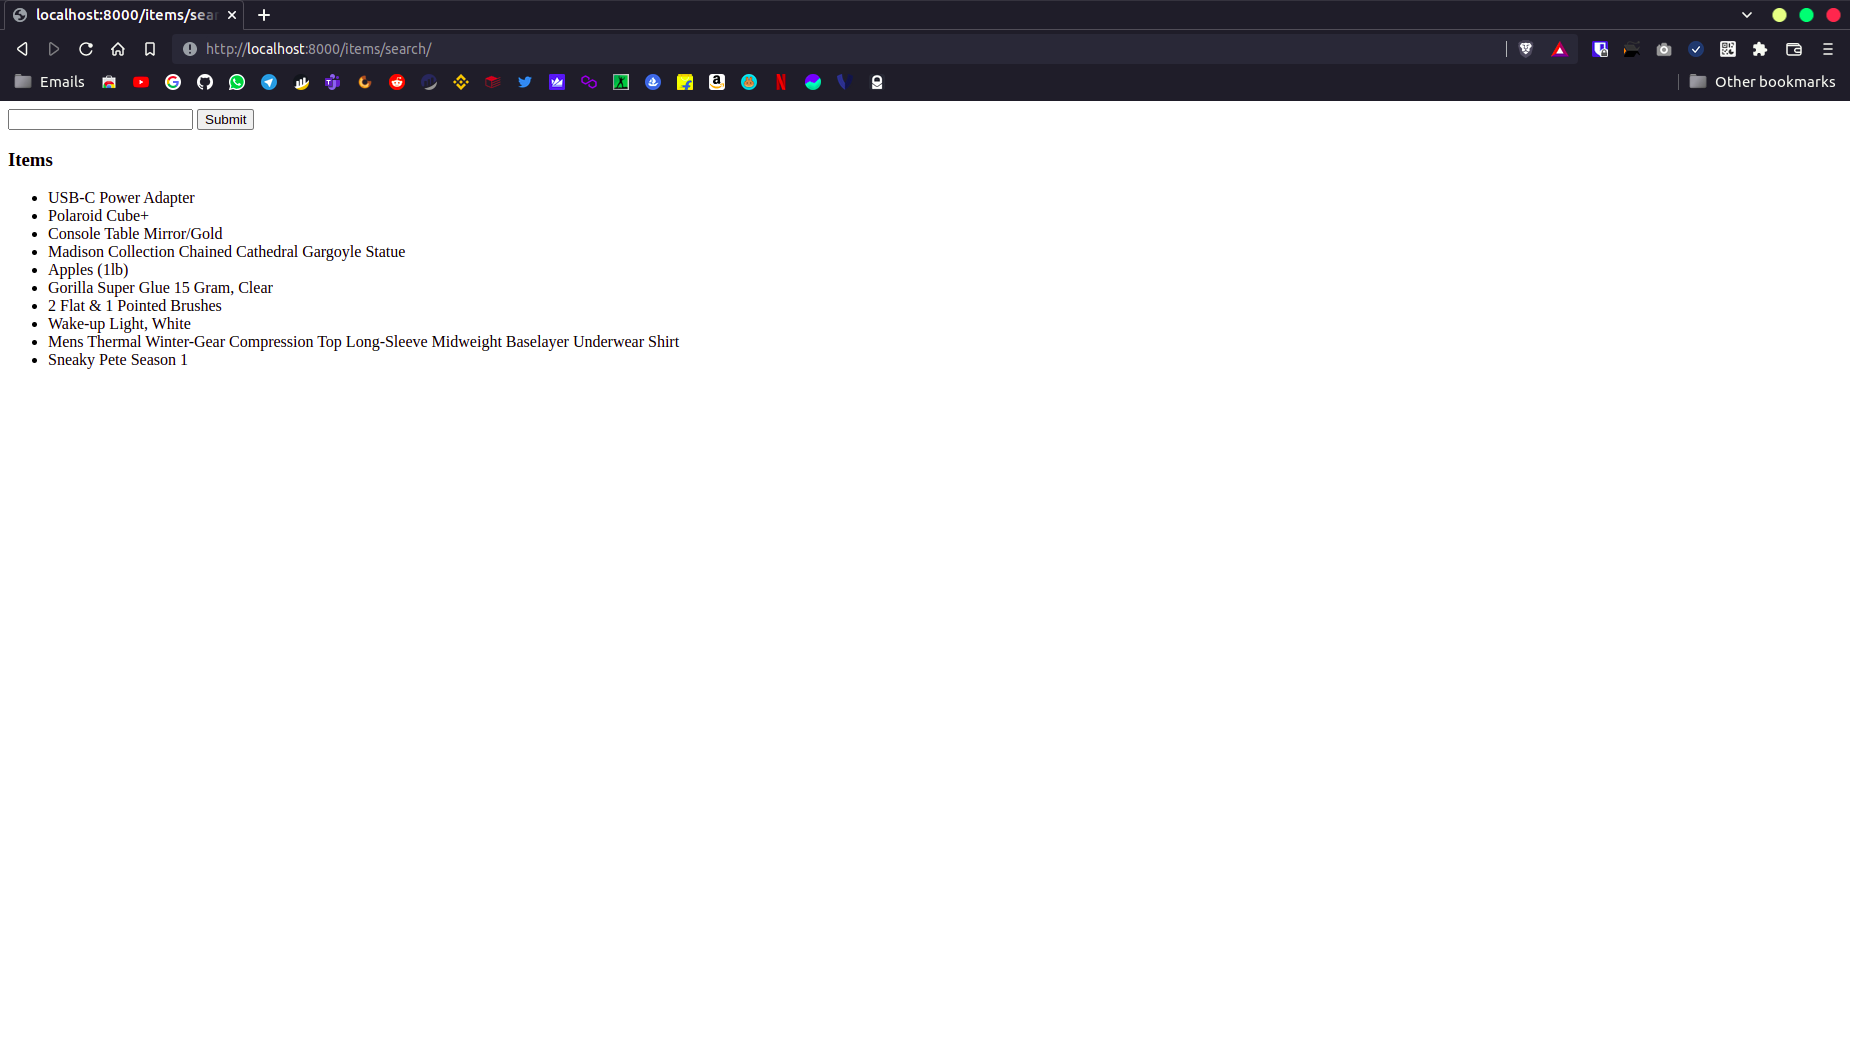
\includegraphics[scale=0.25]{sql_before}
	\captionof{figure}{Item Search Page}
\end{center}

\noindent
SQL Injection query: \\'UNION SELECT password FROM auth\_user WHERE first\_name LIKE'
\begin{center}
	\vspace{0.1cm}
	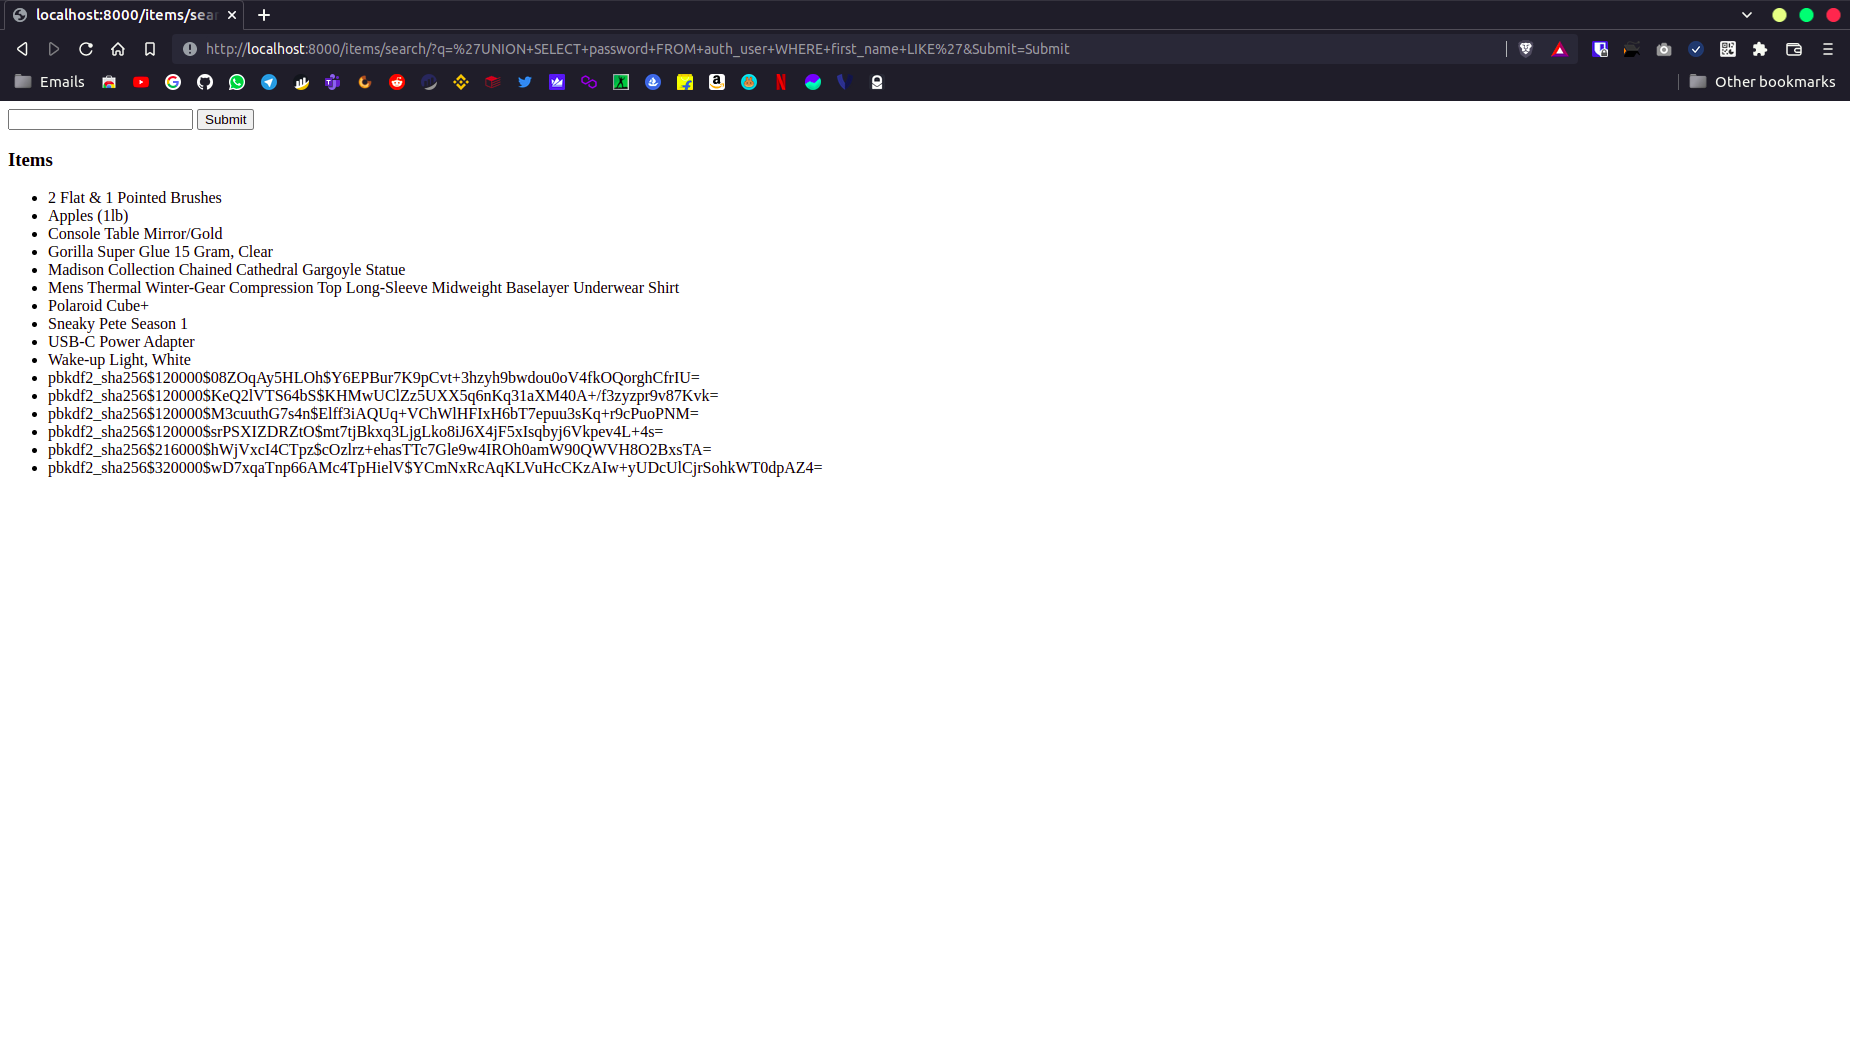
\includegraphics[scale=0.25]{sql_after}
	\captionof{figure}{Unauthorised access of data}
\end{center}

\begin{center}
	\vspace{0.1cm}
	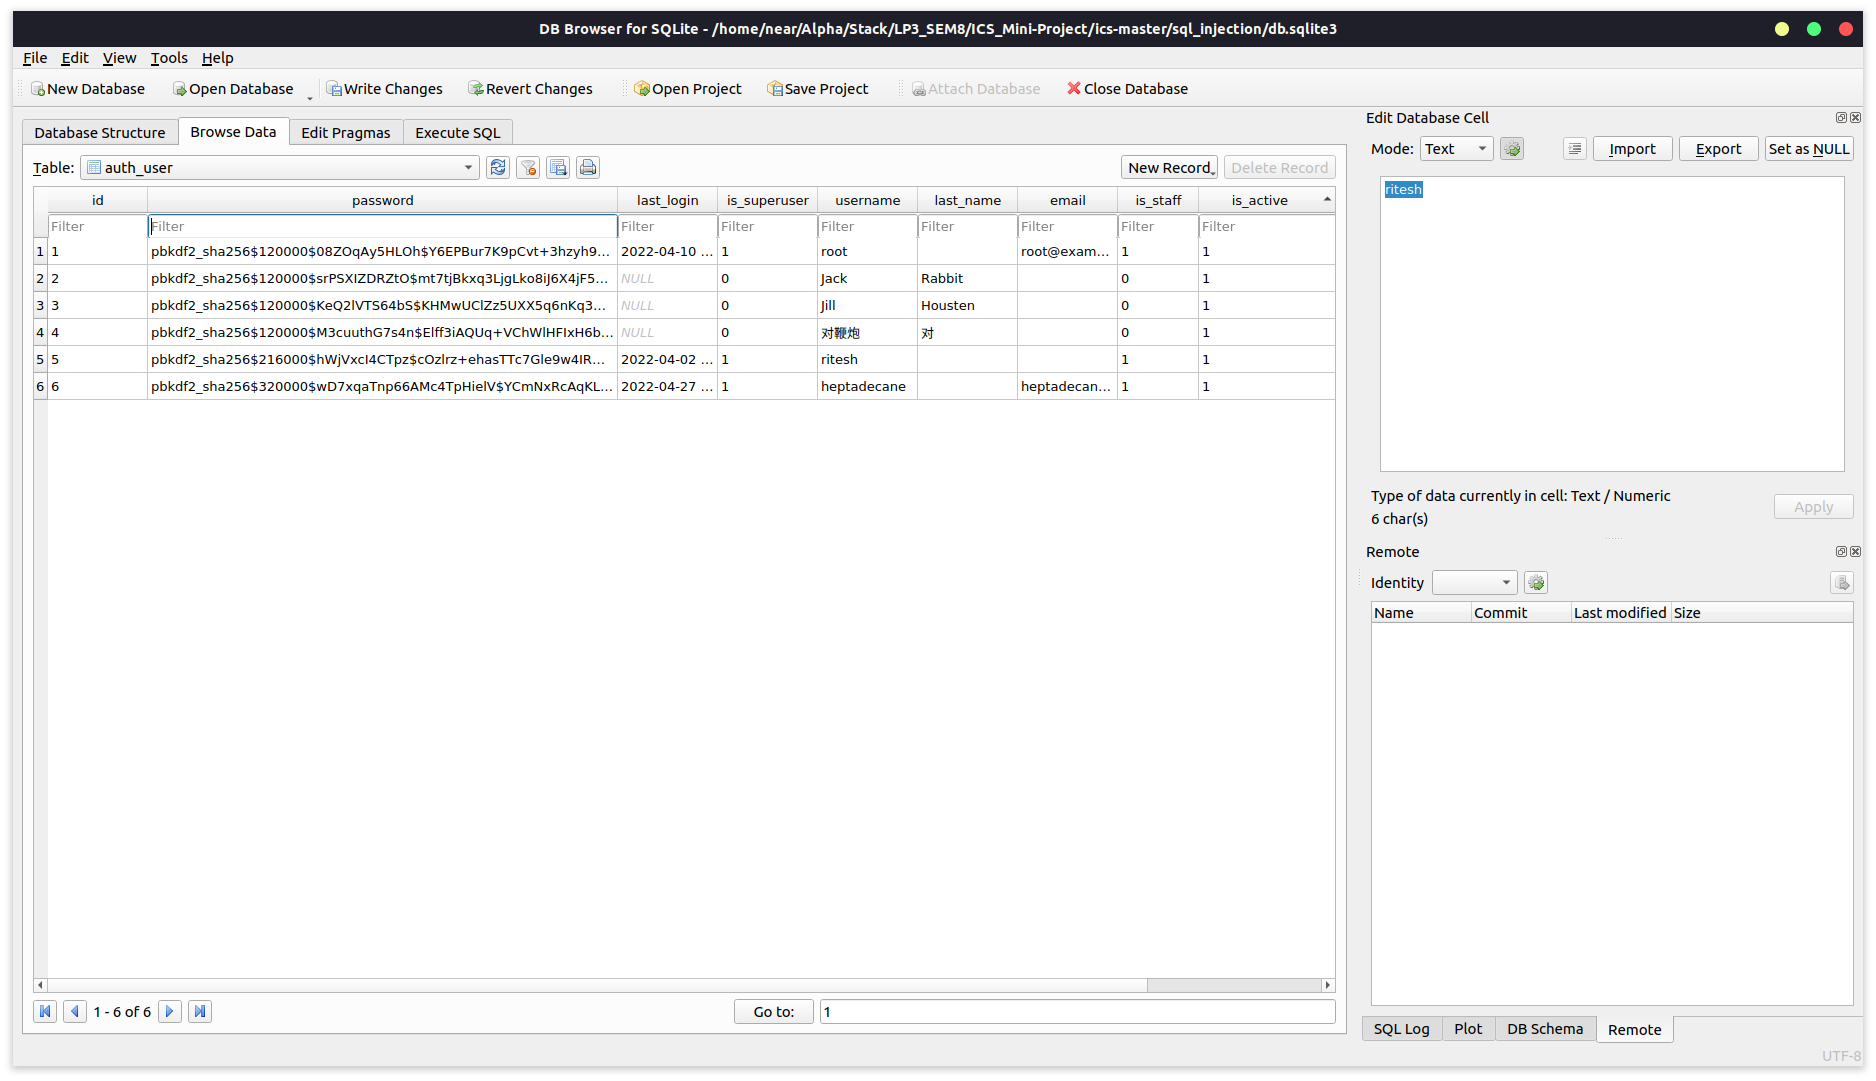
\includegraphics[scale=0.25]{sql_db}
	\captionof{figure}{SQLite: auth\_user table}
\end{center}

\noindent
2. XSS Attack:

\begin{center}
	\vspace{0.1cm}
	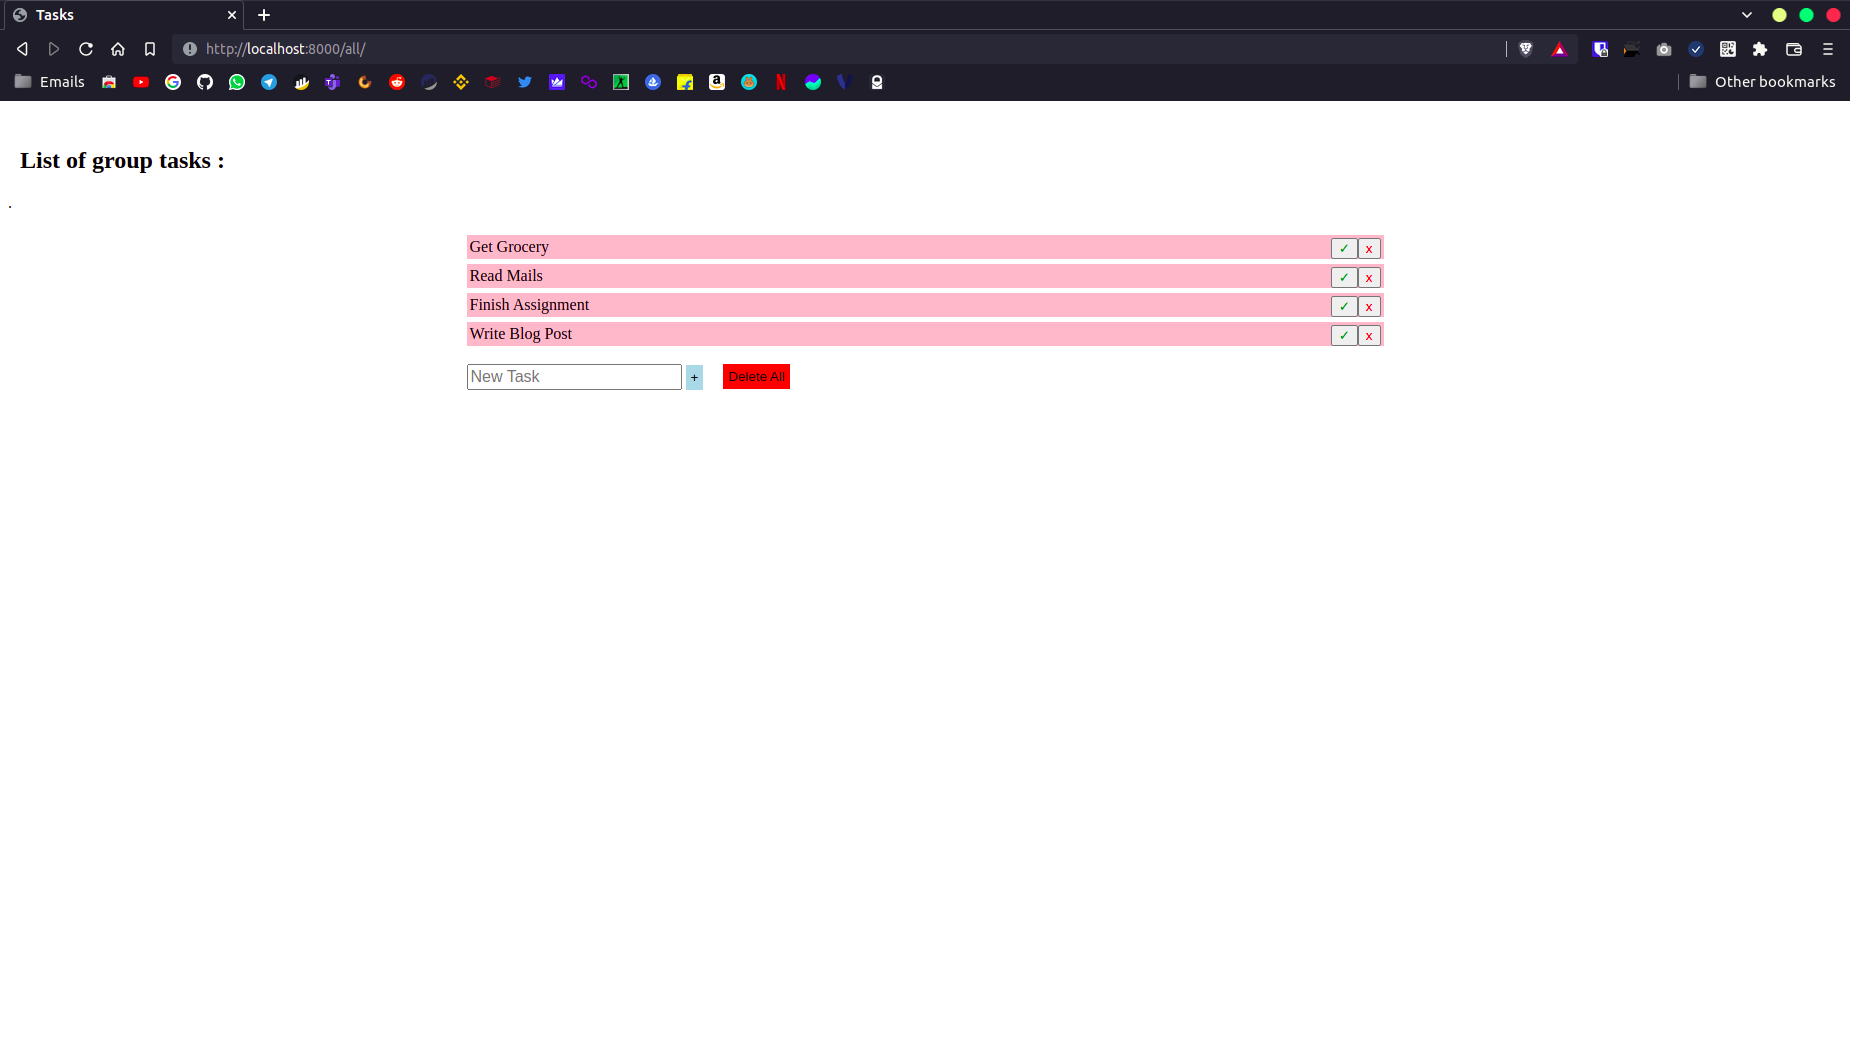
\includegraphics[scale=0.25]{xss_before}
	\captionof{figure}{ToDo List}
\end{center}

\newpage
\noindent
XSS Script: \\
<pre><code> \\
Malicious Code \\
<form id="myform" action="http://127.0.0.1:8000/deleteall" method="post"></form> \\
<script>setTimeout(() => {document.getElementById("myform").submit();}, 5000);</script>\\
</code></pre>
\begin{center}
	\vspace{0.1cm}
	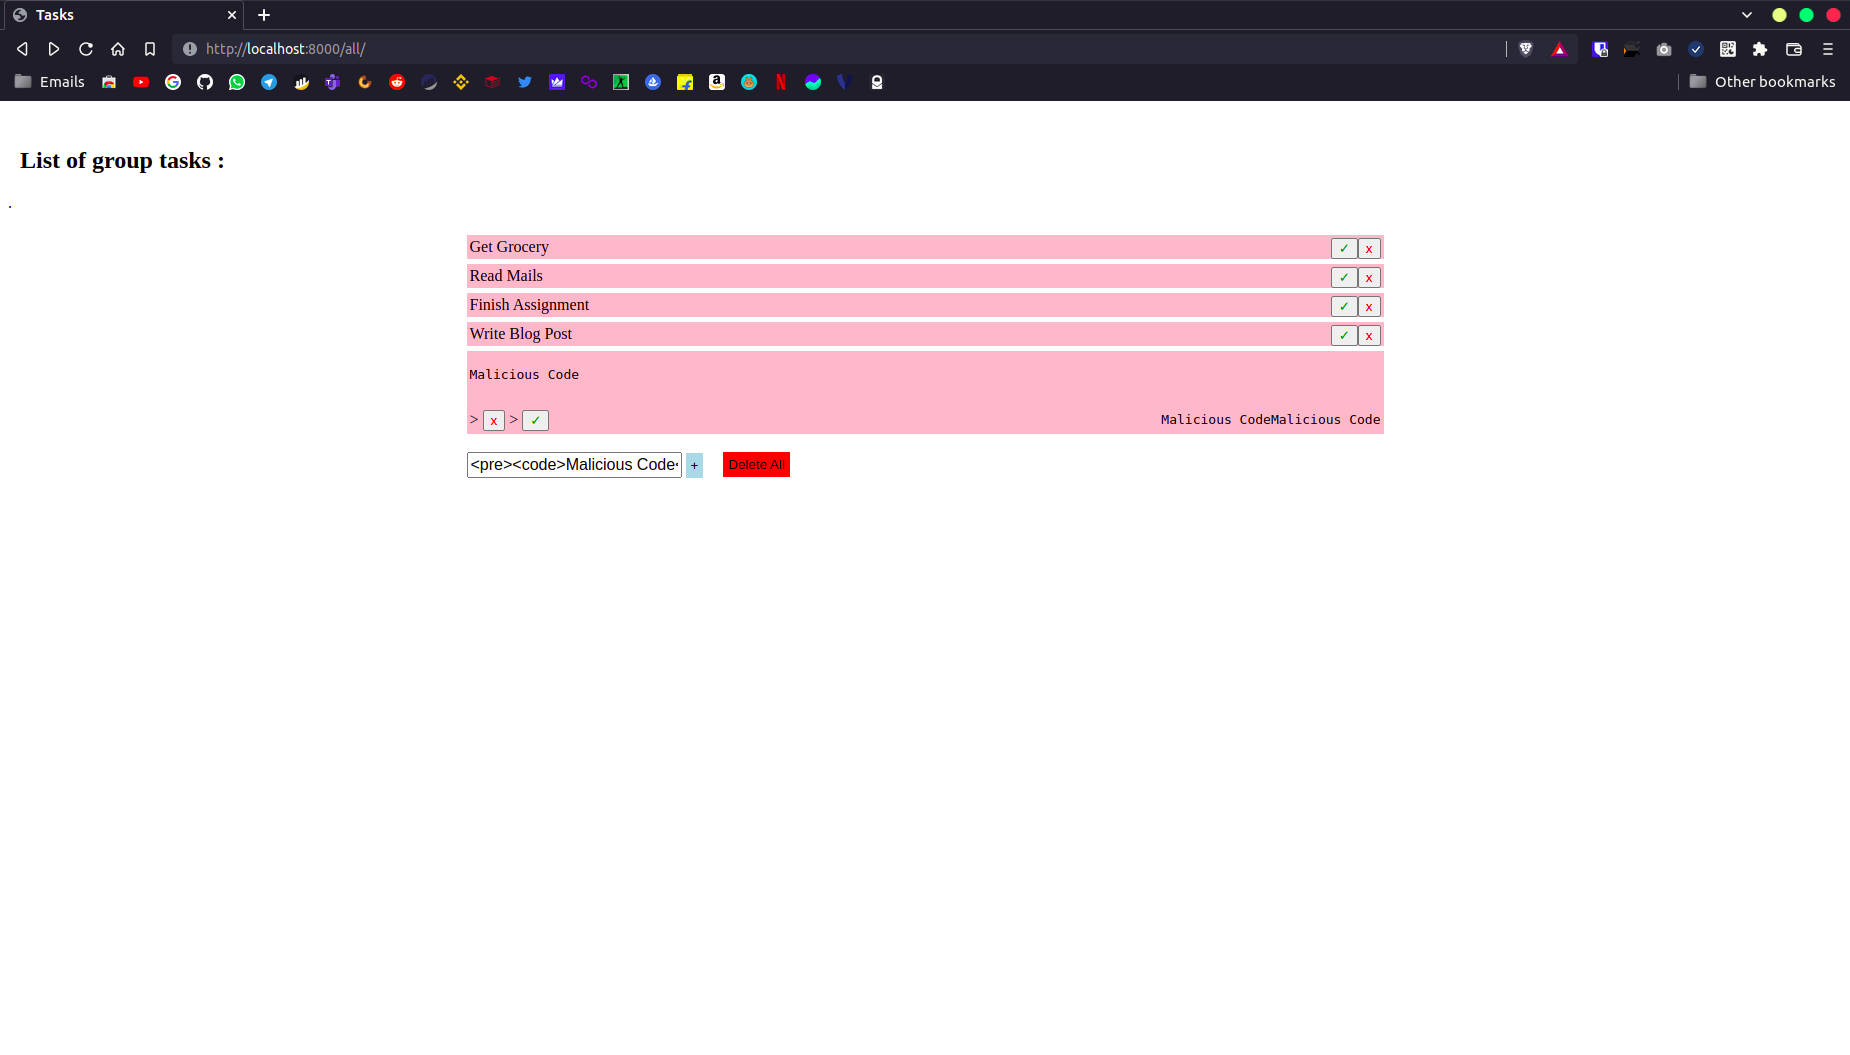
\includegraphics[scale=0.25]{xss_after}
	\captionof{figure}{Malicious snippet to POST 'deleteall'}
\end{center}

\begin{center}
	\vspace{0.1cm}
	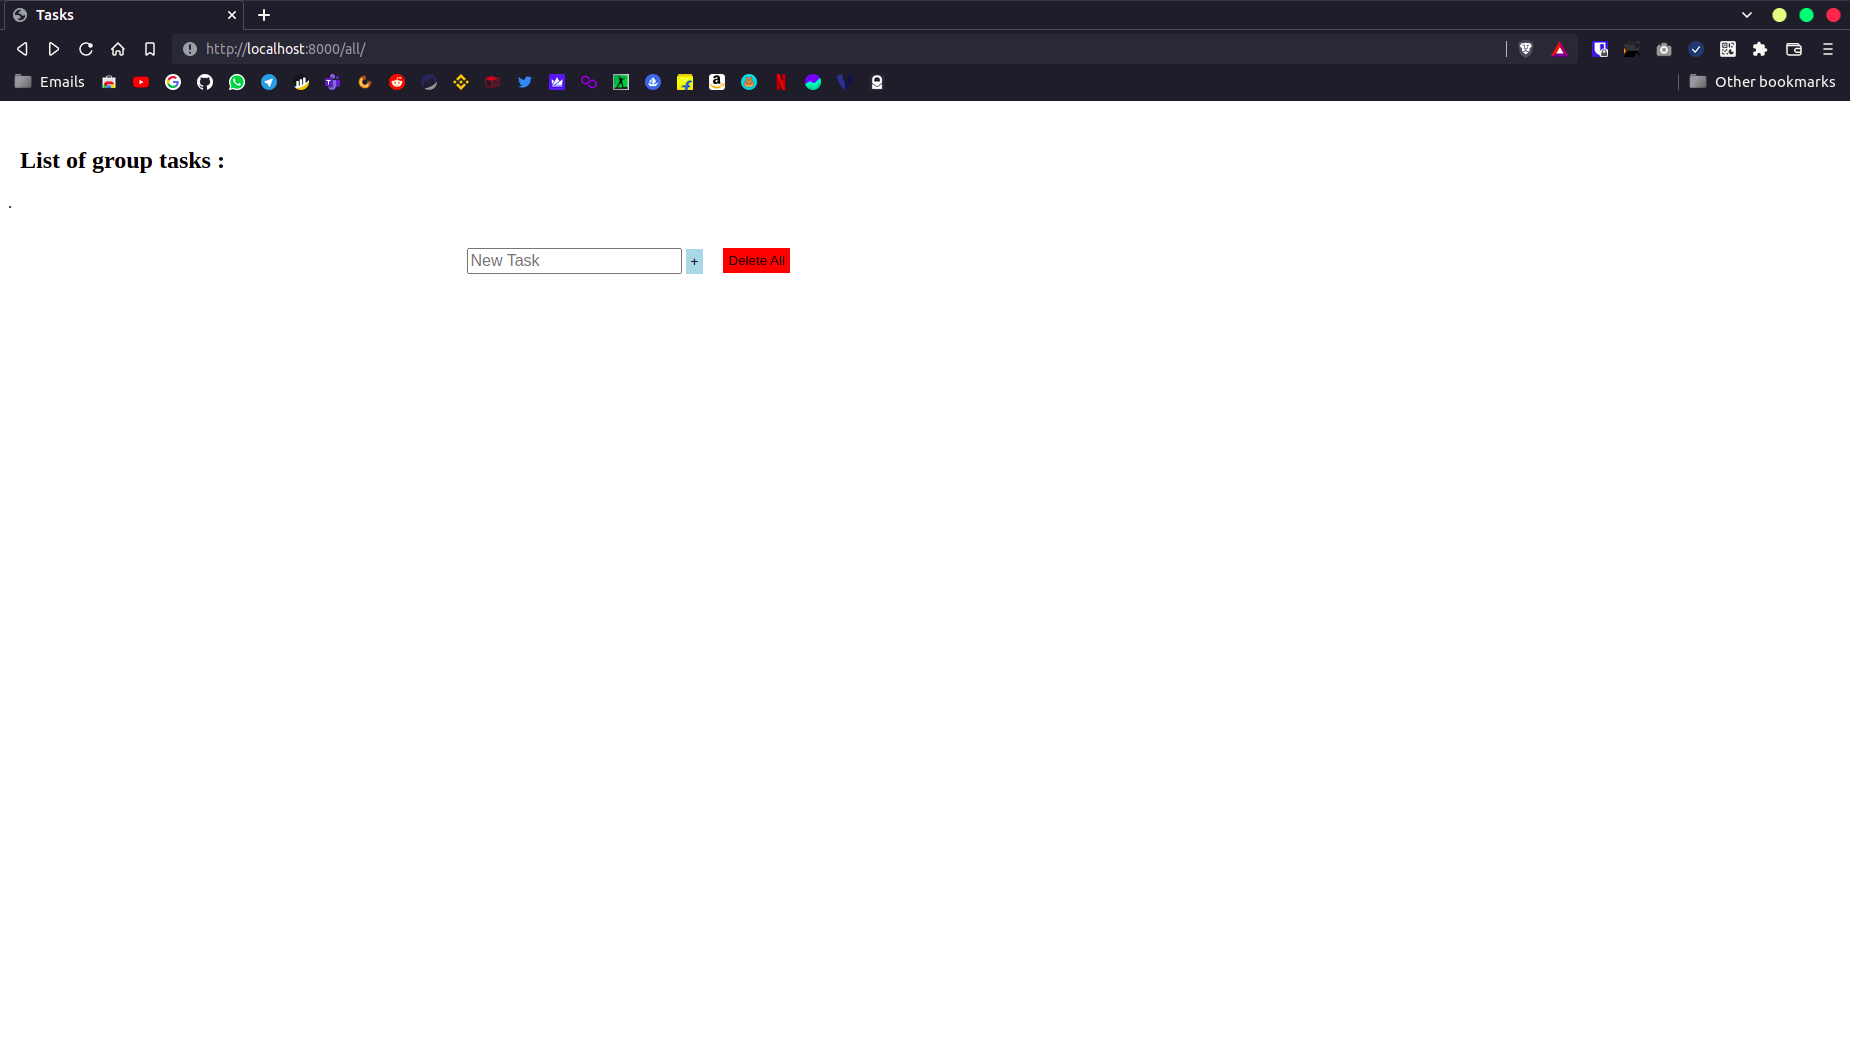
\includegraphics[scale=0.25]{xss_affect}
	\captionof{figure}{Items deleted due to Malicious script}
\end{center}

\newpage
\begin{center}
	\vspace{0.1cm}
	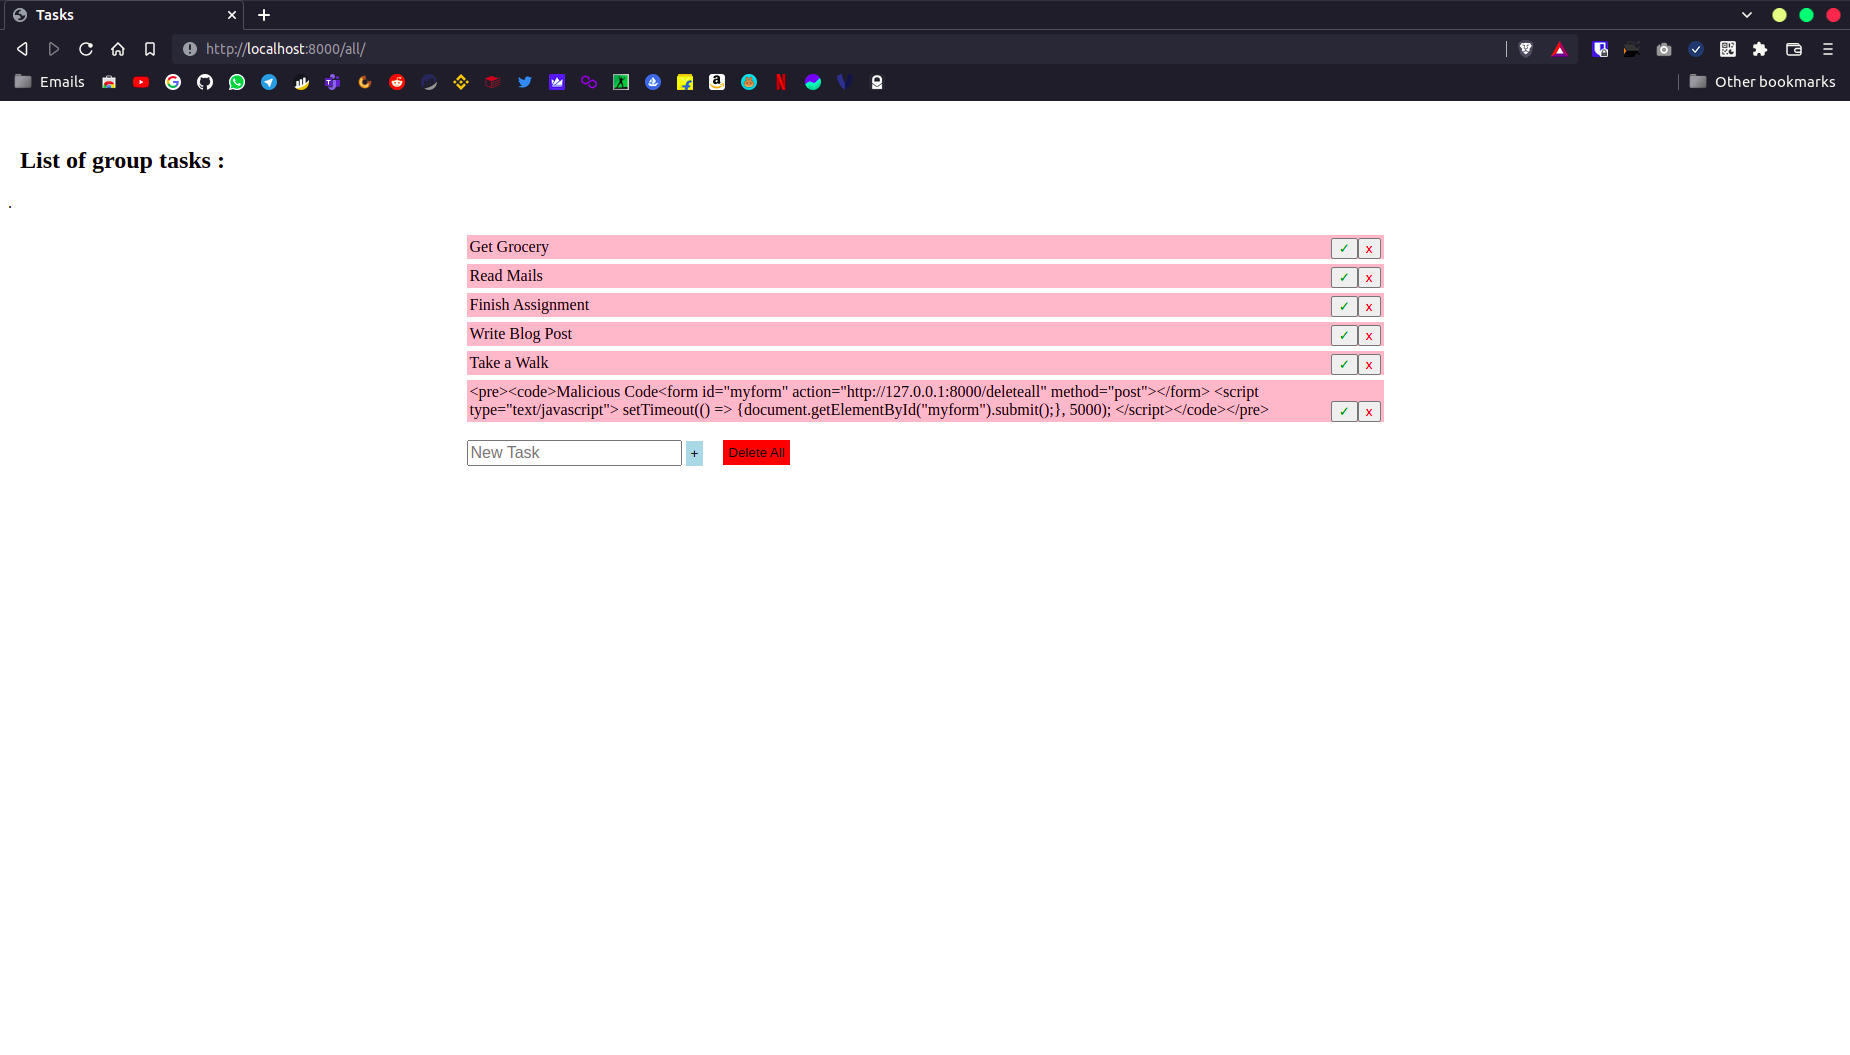
\includegraphics[scale=0.25]{xss_prevent}
	\captionof{figure}{Preventing XSS sxripts with escaping/encoding}
\end{center}

\noindent
\\
\textbf{Conclusion:} \\
With this study, we have successfully demonstrated SQL Injection and Cross-Site Scripting attacks.
Also, designed a website demonstrating prevention and detection of the discussed attacks. \\


\end{document}

